\chapter{Le tenseur des contraintes} \label{chap:Ch02}
\section{Notions générales} \label{sec:Ch02-1}
\subsection{Vecteur contrainte tenseur des contraintes} \label{ssec:Ch02-1.1}
\begin{multicols}{2}
    \begin{center}
        \psfrag{D}{$D$}
        \psfrag{O}{$\Omega$}
        \psfrag{M1}{$M_1$}
        \psfrag{M2}{$M_2$}
        \psfrag{n}{$\vec{n}$}
        \psfrag{df}{$\vec{\ud f}$}
        \psfrag{T}{$\vec{T}$}
        \psfrag{Tt}{$\vec{T}_t$}
        \psfrag{Tn}{$\vec{T}_n$}
    \includegraphics{../images/T1_Ch02-0001}
    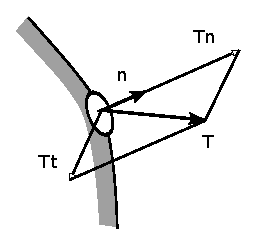
\includegraphics{../images/T1_Ch02-0002}
    \end{center}
\end{multicols}
Le vecteur contrainte caractérise les efforts de contact exercés à travers un élément de surface $\ud S$ de normale $\vec{n}$ sur une partie $D$ du milieu continu: le vecteur contrainte est défini par
\begin{equation}
    \vec{T}(\vec{n}) = \lim_{\ud S \rightarrow D} \frac{\ud \vec{f}}{\ud S} \qquad \ud \vec{f} = \vec{T}\left( \vec{n} \right) \ud D
    \label{eq:Ch02-001}
\end{equation}
Suivant le cas, il s'agit des efforts exercés sur $D$ par le reste du milieu continu (point $M_1$ -- il s'agit alors pour le solide $\Omega$ d'un effort intérieur) ou bien par l'extérieur (point $M_2$ -- effort extérieur pour $\Omega$).

Par convention on choisit pour $\vec{n}$ la normale extérieure au domaine $D$ sur lequel s'applique $\vec{T}$. 
Cette convention est à peu près universelle en MMC, à une exception près: la Mécanique des Sols, où l'on utilise la convention contraire.
Par convention également, on prend, en Mécanique des Solides, le zéro des contraintes pour la pression atmosphérique.
Les contraintes sont donc mesurées par rapport à cette pression atmosphérique.
Ainsi, si le solide est en contact avec un fluide à la pression $p$:
\begin{multicols}{3}
    \centering
    \psfrag{n}{$\vec{n}$}
    \psfrag{T}{$\vec{T}$}
    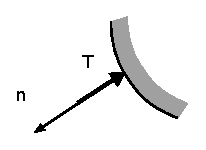
\includegraphics{../images/T1_Ch02-0003a}\\
    $p > p_{atm}$
    \columnbreak

    \psfrag{T}[c]{$\vec{T}=0$}
    
\includegraphics{../images/T1_Ch02-0003b}\\
    $p = p_{atm}$
    \columnbreak

    \psfrag{T}{$\vec{T}$}
    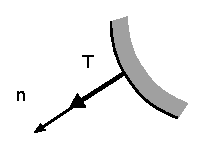
\includegraphics{../images/T1_Ch02-0003c}\\
    $p < p_{atm}$
\end{multicols}
\begin{equation}
    \vec{T} = -\left( p - p_{atm} \right) \vec{n}
    \label{eq:Ch02-002}
\end{equation}
La pression atmosphérique est d'ailleurs en général négligeable par rapport aux contraintes que l'on rencontre.

On projette le vecteur contrainte sur la normale et sur le plan perpendiculaire
\begin{equation}
    \vec{T} = T_{n}\vec{n} + \vec{T}_{t}
    \label{eq:Ch02-003}
\end{equation}
$T_n$ est la contrainte normale (algébrique), $\vec{T}_t$ est la contrainte tangentielle ou de cisaillement. 

Le vecteur contrainte est associé à un élément de surface de normale extérieure $\vec{n}$ -- on parle en général d'une «~facette~». 
Pour connaître «~l'état de contrainte~» en un point donné, il faut connaître les vecteurs contraintes associés à toutes les facettes, c'est à dire à tout vecteur unitaire $\vec{n}$.
Ici intervient le Lemme~\ref{lem:Ch01-2} du paragraphe~\ref{ssec:Ch01-1.2} qui permet de montrer que $\vec{T}$ dépend linéairement de $\vec{n}$.
Il existe donc une application linéaire -- le «~tenseur des contraintes~» -- faisant passer de $\vec{n}$ à $\vec{T}$
\begin{equation}
    \vec{T} = \mathbb{\sigma} \vec{n}
    \label{eq:Ch02-004}
\end{equation}
Le tenseur des contraintes est donc une application linéaire de l'espace vectoriel à trois dimensions $E_3$ dans lui-même.
Si l'on choisit une base orthonormée $\vec{e}_i$, cette application linéaire est représentée par une matrice d'éléments $\sigma_{ij}\ (i,\ j = 1,\ 2,\ 3)$  et la relation~\eqref{eq:Ch02-004} donne la relation matricielle
\begin{equation*}
    \begin{bmatrix}
        T_1\\
        T_2\\
        T_3
    \end{bmatrix}
    =
    \begin{bmatrix}
        \sigma_{11} & \sigma_{12} & \sigma_{13}\\
        \sigma_{21} & \sigma_{22} & \sigma_{23}\\
        \sigma_{31} & \sigma_{32} & \sigma_{33}
    \end{bmatrix}
    \begin{bmatrix}
        n_1\\
        n_2\\
        n_3
    \end{bmatrix}
\end{equation*}
c'est à dire \eqref{eq:Ch01-014}.
On obtient ensuite les équations d'équilibre \eqref{eq:Ch01-017} et la symétrie du tenseur des contraintes \eqref{eq:Ch01-019} à partir de la loi fondamentale. 
En d'autres termes, et c'est ce point de vue que l'on trouvera dans les traités classiques, on obtient~\eqref{eq:Ch02-004} en écrivant l'équilibre d'un tétraèdre, et en écrivant l'équilibre d'un parallélépipède on obtient 
\begin{itemize}
    \item à partir de l'équation de résultante, les équations d'équilibre~\eqref{eq:Ch01-017};
    \item à partir de l'équation de moment, la symétrie du tenseur des contraintes
\end{itemize}

De manière similaire, si $\Sigma$ est une surface de discontinuité -- par exemple une interface entre deux matériaux différents -- alors, l'équilibre d'un disque aplati parallèle à $\Sigma$ donne la condition~\eqref{eq:Ch01-022} de continuité du vecteur contrainte associé à $\Sigma$
\begin{equation}
    \sigma_{ij}^+ N_j = \sigma_{ij}^- N_j
    \label{eq:Ch02-005}
\end{equation}

Si l'on considère un second repère orthonormé $\vec{e}_i^{\prime}$ relié au premier par une matrice de passage $Q_{ij}$ orthogonale
\begin{equation}
    \vec{e}_i^{\prime} = Q_{ij} \vec{e}_j,\ Q_{ij}Q_{ik} = Q_{ji}Q_{ki} = \delta_{jk}
    \label{eq:Ch02-006}
\end{equation}
alors les composantes des vecteurs $\vec{T}$ et $\vec{n}$ et d'un tenseur $\sigma_{ij}$ se transforment (Annexe~\ref{Ann:A}) par
\begin{equation}
    T_i^{\prime} = Q_{ij} T_j,\ \sigma_{ij}^{\prime} = Q_{ik}Q_{jl} \sigma_{kl}
    \label{eq:Ch02-007}
\end{equation}

Les composantes $\sigma_{11}$, $\sigma_{22}$, $\sigma_{13}$, \dots sont les composantes des vecteurs contraintes associés aux facettes normales à $\vec{e}_1$, $\vec{e}_2$, $\vec{e}_3$.
\begin{multicols}{2}
    \begin{center}
        \psfrag{x1}{$x_1$}
        \psfrag{x2}{$x_2$}
        \psfrag{x3}{$x_3$}
        \psfrag{s11}{$\sigma_{11}$}
        \psfrag{s12}{$\sigma_{12}$}
        \psfrag{s13}{$\sigma_{13}$}
        \psfrag{s23}{$\sigma_{23}$}
        \psfrag{s22}{$\sigma_{22}$}
        \psfrag{s33}{$\sigma_{33}$}
        \includegraphics{../images/T1_Ch02-0004}
    \end{center}
    \columnbreak
    \begin{center}
        \psfrag{x1}{$x_1$}
        \psfrag{x2}{$x_2$}
        \psfrag{s11}{$\sigma_{11}$}
        \psfrag{s12}{$\sigma_{12}$}
        \psfrag{s22}{$\sigma_{22}$}
        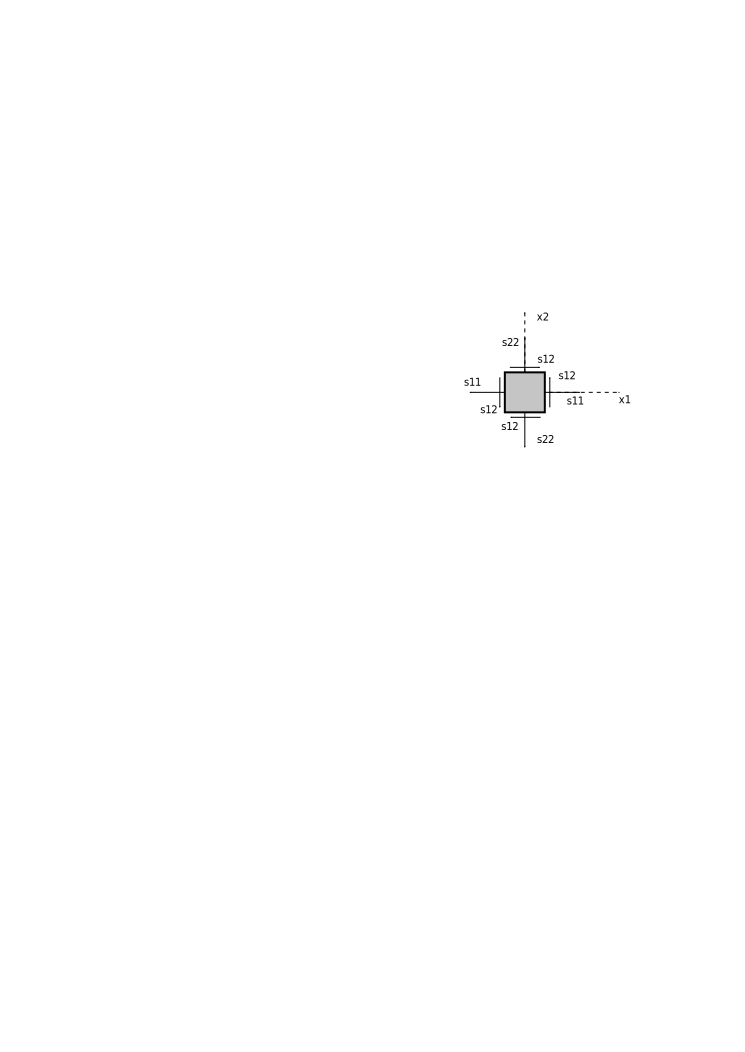
\includegraphics{../images/T1_Ch02-0005}
    \end{center}
\end{multicols}
Les composantes diagonales $\sigma_{11}$, $\sigma_{22}$, $\sigma_{33}$, sont donc des contraintes normales, tandis que les composantes non diagonales $\sigma_{12}$, $\sigma_{13}$, \dots sont des contraintes de cisaillement.
La symétrie du tenseur des contraintes $\sigma_{12} = \sigma_{21}$ exprime l'égalité de la contrainte de cisaillement associée à deux facettes perpendiculaires.
Peur cette raison, cette symétrie est souvent appelée «~principe de réciprocité des cisaillements~».

Dimensionnellement, une «~contrainte~» -- qu'il s'agisse d'une composante du vecteur contrainte ou du tenseur des contraintes -- est homogène à une force par unité de surface, donc à une pression.
L'unité SI, le Pascal ($1 Pa = 1 N/m^2$) étant très petite par rapport aux contraintes habituellement rencontrées, on utilise traditionnellement l'hectobar, le mégapascal et le $daN/mm$ (et chez les anglo-saxons, le p.s.i. \textit{pound per square inch}).
\begin{itemize}
    \item[] 1 daN/mm$^2$ = 1 hectobar = 10 MPa = $10^7$ Pa
\end{itemize}

\subsection{Contraintes principales invariants} \label{ssec:Ch02-1.2}
Le tenseur des contraintes est symétrique; on peut donc le diagonaliser.
Il existe trois directions principales orthogonales associées à trois valeurs propres $\sigma_1$, $\sigma_2$, $\sigma_3$,  appelées «~contraintes principales~».
\begin{equation}
    \sigma_{ij} e_j^{(1)} = \sigma_1 e_i^{(1)},\ \text{ etc.}
    \label{eq:Ch02-008}
\end{equation}
À partir de la décomposition~\eqref{eq:Ch02-003}, on voit qu'une condition nécessaire et suffisante pour qu'une direction soit principale pour $\mathbb{\sigma}$ est que la contrainte exercée sur la facette correspondante soit purement normale (pas de contrainte de cisaillement).
Dans le repère principal, la matrice représentative du tenseur des contraintes est diagonale.
Par abus de langage, on dit que le tenseur des contraintes est diagonal, et on écrit
\begin{equation}
    \mathbb{\sigma} = 
    \begin{bmatrix}
        \sigma_1 & 0 & 0 \\
        0 & \sigma_2 & 0 \\
        0 & 0 & \sigma_3
    \end{bmatrix}
    \label{eq:Ch02-009}
\end{equation}

Les contraintes principales s'obtiennent par résolution de l'équation caractéristique 
\begin{align}
    P_{\mathbb{\sigma}} & = \det
    \begin{bmatrix}
        \sigma_{11}-\lambda & \sigma_{12} & \sigma_{13}\\
        \sigma_{12} & \sigma_{22}-\lambda & \sigma_{23}\\
        \sigma_{13} & \sigma_{22} & \sigma_{33}-\lambda
    \end{bmatrix} \nonumber \\ 
        & = -\lambda^3 + I_1 \lambda^2 - I_2 \lambda + I_3
    \label{eq:Ch02-010}
\end{align}
où $I_1$, $I_2$, $I_3$	sont les invariants de $\mathbb{\sigma}$ définis par (Annexe~\ref{Ann:A})
\begin{equation}
    \left\{
    \begin{aligned}
        I_1 &= \sigma_{ii}= \sigma_1 + \sigma_2 + \sigma_3\\
        I_2 &= \frac{1}{2}\left( \sigma_{ii}\sigma_{jj} - \sigma_{ij}\sigma_{ij} \right) = \sigma_1\sigma_2 + \sigma_2\sigma_3 + \sigma_3\sigma_1\\
        I_3 &= \det \left( \sigma_{ij} \right) = \sigma_1\sigma_2\sigma_3
    \end{aligned}
    \right.
    \label{eq:Ch02-011}
\end{equation}
On 	décompose habituellement le tenseur des contraintes en déviateur et partie sphérique
\begin{equation}
    \sigma_{ij} = \sigma \delta_{ij} + s_{ij}
    \label{eq:Ch02-012}
\end{equation}
où  $\sigma$ est la partie sphérique
\begin{equation}
    \sigma = \frac{1}{3}I_1 = \frac{\sigma_{11} + \sigma_{22} + \sigma_{33}}{3} = \frac{\sigma_1 + \sigma_2 + \sigma_3}{3}
    \label{eq:Ch02-013}
\end{equation}
et où $s_{ij}$ est le déviateur (on appelle déviateur un tenseur de trace nulle)
\begin{equation}
    \left\{
    \begin{aligned}
        & s_{ii} = 0 \qquad s_{ij} = \sigma_{ij} + \frac{1}{3} \sigma_{kk} \delta_{ij}\\
        & s_{12} = \sigma_{12} \qquad s_{11}= \frac{2\sigma_{11} - \sigma_{22} -\sigma_{33}}{3}
    \end{aligned}
    \right.
    \label{eq:Ch02-014}
\end{equation}
Il est clair que le tenseur des contraintes et son déviateur ont mêmes directions principales, les contraintes principales déviatoires $s_1$, $s_2$, $s_3$ sont données par 
\begin{equation}
    s_1 = \frac{2\sigma_1 - \sigma_2 - \sigma_3}{3}
    \label{eq:Ch02-015}
\end{equation}
et les invariants $J_2$, $J_3$ (puisque $J_1 = 0$ par~\eqref{eq:Ch02-014}) du déviateur $s_{ii}$ sont donnés par 
\begin{equation}
    \left\{
    \begin{aligned}
        J_2 &= -\frac{1}{2}s_{ij}s_{ij}\\
        &= s_1 s_2 + s_2 s_3 + s_3 s_1\\
        &= -\frac{1}{2} \left( s_1^2 + s_2^2 + s_3^2 \right)\\
        &= -\frac{1}{6} \left[ \left( \sigma_1 - \sigma_2 \right)^2 + \left( \sigma_2 - \sigma_3 \right)^2 + \left( \sigma_3 -\sigma_1 \right)^2 \right]\\
        J_3 &= \det \left( s_{ij} \right)  = s_1 s_2 s_3
    \end{aligned}
    \right.
    \label{eq:Ch02-016}
\end{equation}
\subsection{États de contraintes particuliers} \label{ssec:Ch02-1.3}
Nous allons envisager divers cas particuliers correspondant à des états de contraintes remarquables. 
\subsubsection{État de tension ou compression hydrostatique}
\begin{equation}
    \mathbb{\sigma} = 
    \begin{bmatrix}
        \sigma & 0 & 0 \\
        0 & \sigma & 0 \\
        0 & 0 & \sigma
    \end{bmatrix}
    \begin{aligned}
        \text{tension si } & \sigma > 0\\
        \text{compression si } & \sigma < 0
    \end{aligned}
    \label{eq:Ch02-017}
\end{equation}
Les trois contraintes principales sont égales, le déviateur est nul, et toutes les directions sont principales.
Sur toute facette s'exerce donc une contrainte purement normale.
\begin{multicols}{2}
    \begin{center}
        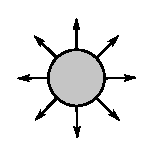
\includegraphics{../images/T1_Ch02-0006a}\\
        $\sigma > 0$ (tension)
    \end{center}
    \columnbreak
    \begin{center}
        \includegraphics{../images/T1_Ch02-0006b}\\
        $\sigma < 0$ (compression)
    \end{center}
\end{multicols}
C'est l'état de contraintes qui existe dans les fluides à l'équilibre, d'où la terminologie «~hydrostatique~».
\subsubsection{État  de  contraintes  de  révolution}
\begin{equation}
    \mathbb{\sigma} = 
    \begin{bmatrix}
        \sigma_1 & 0 & 0 \\
        0 & \sigma_2 & 0 \\
        0 & 0 & \sigma_3
    \end{bmatrix}
    \label{eq:Ch02-018}
\end{equation}
Deux des contraintes principales coïncident; les directions principales sont:
\begin{enumerate}
    \item la direction $x_1$, pour $\sigma_1$;
    \item toute direction du plan $\left( x_2, x_3 \right)$, pour $\sigma_2$.
\end{enumerate}
La décomposition en déviateur et partie sphérique devient 
\begin{equation}
    \mathbb{\sigma} = \sigma 
    \begin{bmatrix}
        1 & 0 & 0\\
        0 & 1 & 0\\
        0 & 0 & 1
    \end{bmatrix}
    +
    s
    \begin{bmatrix}
        1 & 0 & 0\\
        0 & -\frac{1}{2} & 0\\
        0 & 0 & -\frac{1}{2}
    \end{bmatrix},\ 
    \sigma = \frac{\sigma_1 + 2\sigma_2}{3} \quad s = \frac{2\left( \sigma_1 - \sigma_2 \right)}{3}
    \label{eq:Ch02-019}
\end{equation}
\begin{multicols}{2}
    \begin{center}
        \psfrag{s1}{$\sigma_1$}
        \psfrag{s2}{$\sigma_2$}
        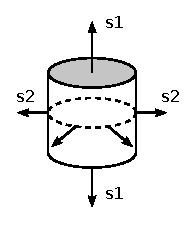
\includegraphics{../images/T1_Ch02-0007a}
    \end{center}
    \columnbreak
    \begin{center}
        \psfrag{s1}{$\sigma_1$}
        \psfrag{s2}{$\sigma_2$}
        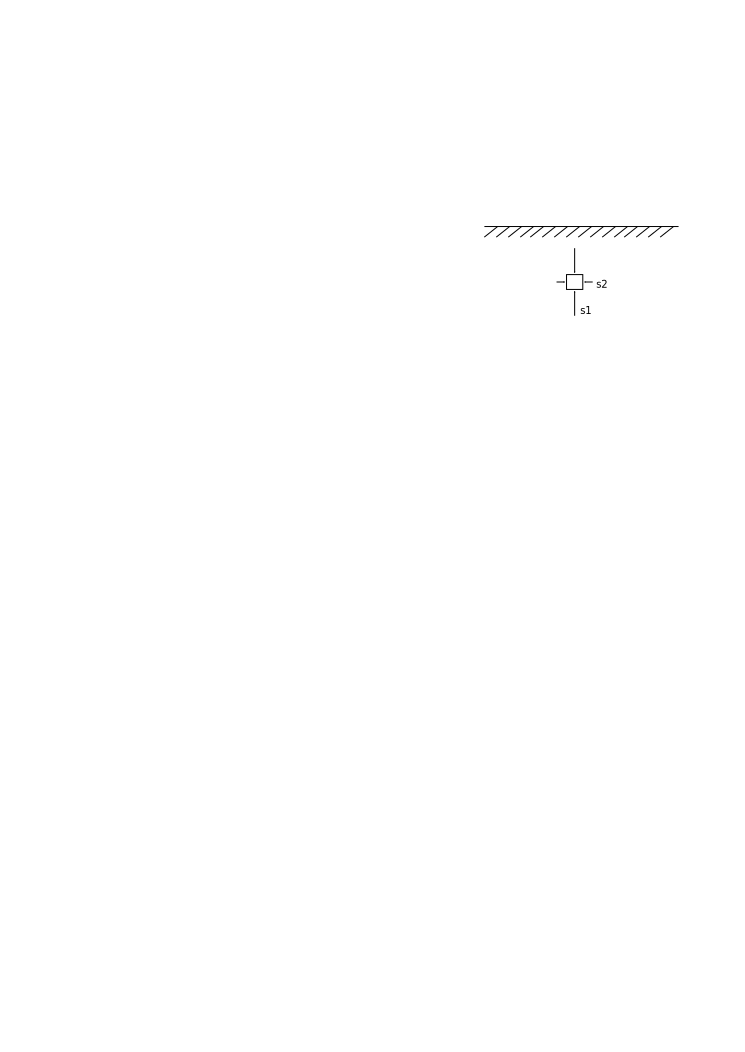
\includegraphics{../images/T1_Ch02-0007b}
    \end{center}
\end{multicols}
C'est l'état de contrainte qui se réalise avec $\sigma_1 <\sigma_2 < 0$ dans le sol en profondeur. 
\subsubsection{État de traction ou compression uniaxiale}
\begin{minipage}[l]{.2\textwidth}
\begin{center}
    \psfrag{s}{$\sigma$}
    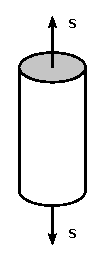
\includegraphics{../images/T1_Ch02-0008}
\end{center}
\end{minipage}
\begin{minipage}[r]{.8\textwidth}
\begin{equation}
    \mathbb{\sigma} = 
    \begin{bmatrix}
        \sigma & 0 & 0 \\
        0 & 0 & 0 \\
        0 & 0 & 0
    \end{bmatrix}
    \begin{aligned}
        \text{traction si } & \sigma > 0\\
        \text{compression si } & \sigma < 0
    \end{aligned}
    \label{eq:Ch02-020}
\end{equation}
C'est un cas particulier du précédent avec $\sigma_2 = 0$ (pas de contrainte latérale). 
C'est l'état de contrainte le plus facile à réaliser expérimentalement: il suffit d'exercer une force longitudinale sur un barreau (essai  de  traction).
\end{minipage}
\subsubsection{État de cisaillement pur}
\begin{equation}
    \mathbb{\sigma} = 
    \begin{bmatrix}
        0 & \tau & 0 \\
        \tau & 0 & 0 \\
        0 & 0 & 0
    \end{bmatrix}
    \label{eq:Ch02-021}
\end{equation}
État de contrainte purement déviatoire.
Les directions principales sont l'axe $x_3$ ($\sigma_3= 0$) et les bissectrices des axes $x_1$, $x_2$ (contraintes principales $+\tau$ et $-\tau$). 
\begin{multicols}{2}
    \begin{center}
        \psfrag{x1}{$x_1$}
        \psfrag{x2}{$x_2$}
        \psfrag{t}{$\tau$}
        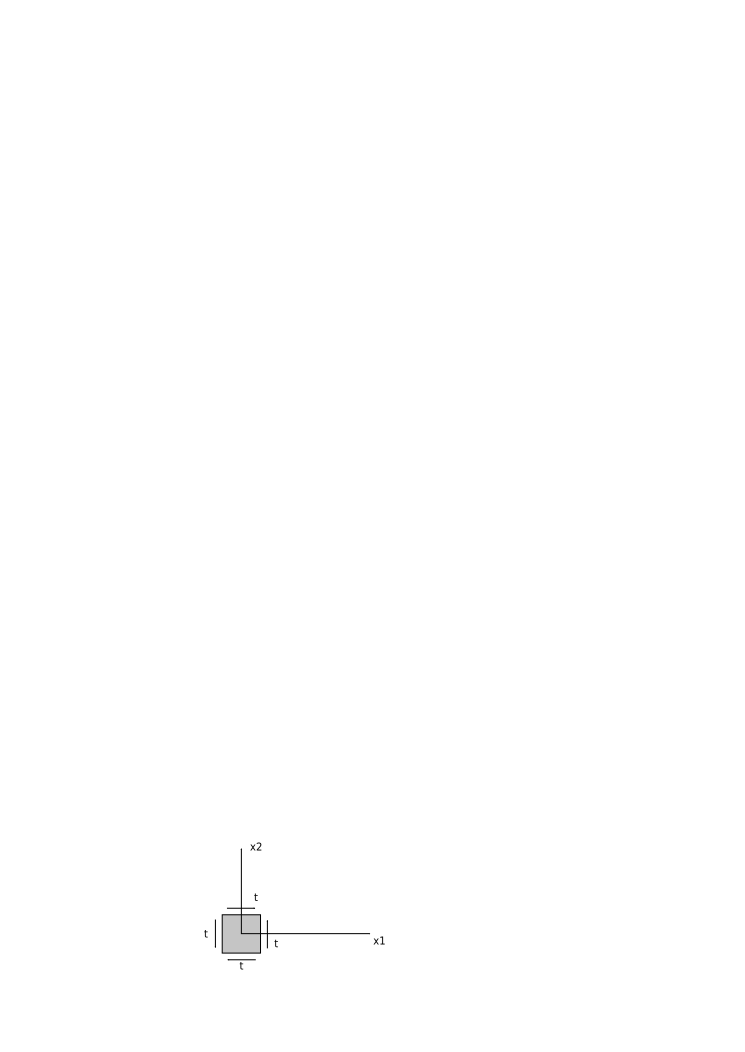
\includegraphics{../images/T1_Ch02-0009a}
    \end{center}
    \begin{center}
        \psfrag{x1}{$x_1$}
        \psfrag{x2}{$x_2$}
        \psfrag{t}{$\tau$}
        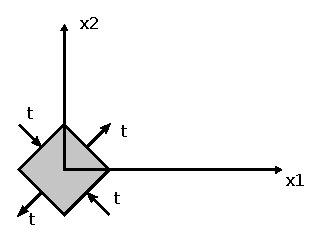
\includegraphics{../images/T1_Ch02-0009b}
    \end{center}
\end{multicols}
\subsubsection{État plan de contraintes}
\begin{equation}
    \mathbb{\sigma} = 
    \begin{bmatrix}
        \sigma_{11} & \sigma_{12} & 0 \\
        \sigma_{12} & \sigma_{22} & 0 \\
        0 & 0 & 0
    \end{bmatrix}
    \text{ ou }
    \begin{bmatrix}
        \sigma_{11} & \sigma_{12} & 0 \\
        \sigma_{12} & \sigma_{22} & 0 \\
        0 & 0 & \sigma_{33}
    \end{bmatrix}
    \label{eq:Ch02-022}
\end{equation}
\begin{minipage}[l]{.3\textwidth}
    \begin{center}
        \psfrag{x1}{$x_1$}
        \psfrag{x2}{$x_2$}
        \psfrag{s11}{$\sigma_{11}$}
        \psfrag{s22}{$\sigma_{22}$}
        \psfrag{s12}{$\sigma_{12}$}
        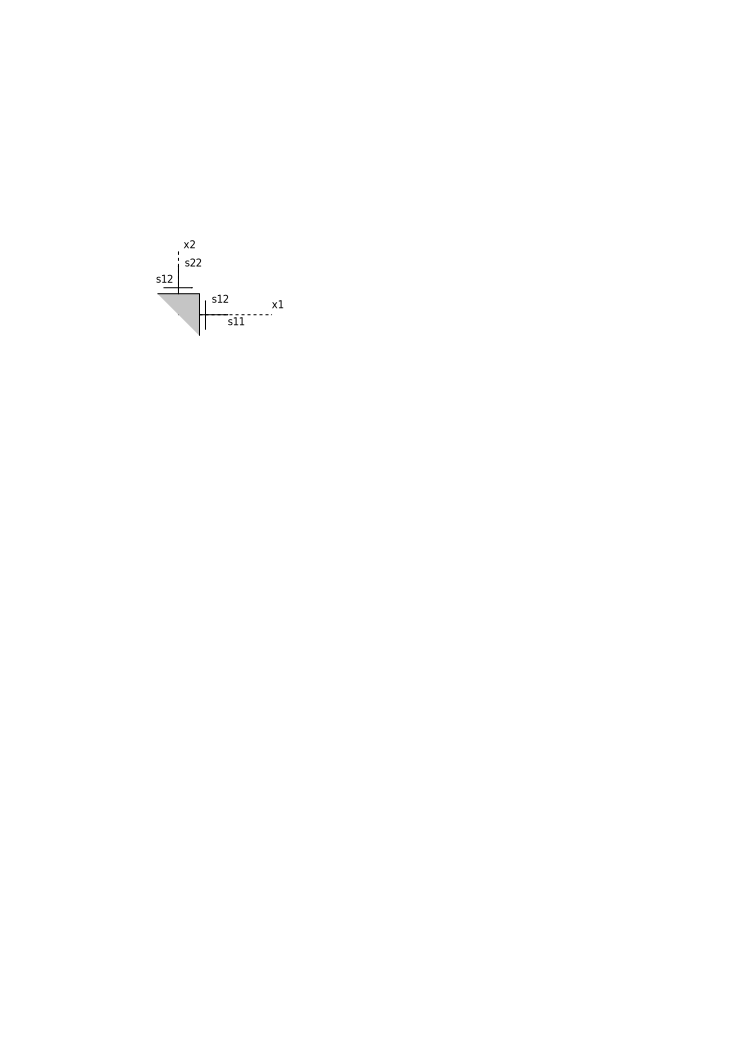
\includegraphics{../images/T1_Ch02-0010}
    \end{center}
\end{minipage}
\begin{minipage}[r]{.7\textwidth}
Les directions principales sont la direction $x_3$ et deux directions perpendiculaires du plan $x_1$, $x_2$.
Lorsque $\vec{n}$ varie dans le plan $x_1$, $x_2$, le vecteur contrainte reste dans le plan, et on peut se limiter au plan $x_1$, $x_2$.
Nous ferons l'étude complète au paragraphe~\ref{ssec:Ch02-3.2}.
\end{minipage}

\section{Représentations géométriques des contraintes} \label{sec:Ch02-2}
L'état de contraintes en un point donné est caractérisé par la valeur en ce point du tenseur des contraintes, c'est à dire par 6 nombres.
Pour visualiser cette entité, on a introduit diverses représentations géométriques.
\subsection{Quadriques des contraintes} \label{ssec:Ch02-2.1}
\subsubsection{Ellipsolde de Lamé}
C'est le lieu de l'extrémité du vecteur contrainte $\vec{T}$ lorsque $\vec{n}$ varie.
Si nous nous plaçons en repère principal, l'équation~\eqref{eq:Ch02-005} donne 
\begin{equation*}
    T_1 = \sigma_1 n_1 \qquad T_2 = \sigma_2 n_2 \qquad T_3 = \sigma_3 n_3
\end{equation*}
et, puisque le vecteur $vec{n}$ est unitaire 
\begin{equation}
    \frac{T_1^2}{\sigma_1^2} + \frac{T_2^2}{\sigma_2^2} + \frac{T_3^2}{\sigma_3^2} = 1
    \label{eq:Ch02-023}
\end{equation}
Le lieu de l'extrémité ($T_1$, $T_2$, $T_3$) est un ellipsoïde d'axes principaux sont les directions principales du tenseur des contraintes et de demi-axe les valeurs absolues des contraintes principales -- c'est l'el1ipsoïde de Lamé.
Mais cet ellipsoïde ne permet pas de visualiser le vecteur contrainte associé à une facette donnée.
\subsubsection{Quadrique directrice des contraintes normales}
Nous considérons la (ou les) quadrique(s) réelle(s) d'équation 
\begin{equation}
    \Phi(x) = \sigma_{ij} x_i x_j = \pm 1
    \label{eq:Ch02-024}
\end{equation}
C'est une (ou deux) quadrique(s) d'axes principaux les directions principales du tenseur des contraintes et de demi-axes ($1/\sqrt{|\sigma_1|}$, \ldots).
On les appelle quadriques directrices des contraintes, car elles permettent de construire le vecteur contrainte associé à une direction $\vec{n}$ quelconque par la construction suivante. 

\noindent\underline{Construction:} On mène de l'origine la demi-droite de direction $\vec{n}$, qui coupe la quadrique en un point $M$.  
\begin{itemize}
    \item la contrainte normale  est donnée  à  partir de  la longueur $OM=\rho$ par
        \begin{equation}
            \rho^2 |T_n| = 1
            \label{eq:Ch02-025}
        \end{equation}
    \item la direction du vecteur contrainte est donnée par la normale $\vec{N}$ à la quadrique en $M$. 
\end{itemize}
\begin{multicols}{2}
    \begin{center}
        \psfrag{x1}{$x_1$}
        \psfrag{x2}{$x_2$}
        \psfrag{x3}{$x_3$}
        \psfrag{n}{$\vec{n}$}
        \psfrag{N}{$\vec{N}$}
        \psfrag{M}{M}
        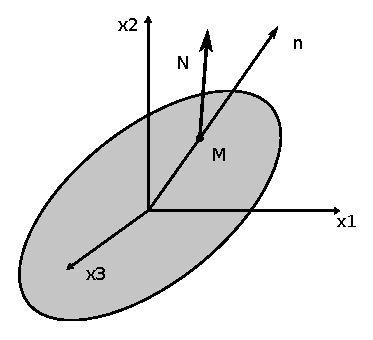
\includegraphics{../images/T1_Ch02-0011}
    \end{center}
    \columnbreak
    \begin{proof}
        On a $\vec{OM} = p \vec{n},\ x_i = p n_i$.
    En reportant dans~\eqref{eq:Ch02-024}, il vient
    \begin{displaymath}
        \rho^2 \sigma_{ij} n_i n_j = \pm 1
    \end{displaymath}
    qui donne~\eqref{eq:Ch02-025}, en remarquant que
    \begin{displaymath}
        T_n = \vec{T} \cdot \vec{n} = \sigma_{ij} n_i n_j
    \end{displaymath}
    La direction de la normale $\vec{N}$ à la quadrique donnée par le gradient de la fonction $\Phi$  est  
    \begin{displaymath}
        N_i = \lambda \frac{\partial \Phi}{\partial x_i} = 2\lambda \sigma_{ij} x_j = 2 \lambda \rho \sigma_{ij} n_j = 2 \lambda \rho T_i
    \end{displaymath}
    et $\vec{N}$ est proportionnel à $\vec{T}$.
    \end{proof}
\end{multicols}
Si toutes les contraintes principales sont de même signe, la forme quadratique 
\begin{equation}
    T_n = \sigma_{ij} n_i n_j
    \label{eq:Ch02-026}
\end{equation}
est définie positive ou négative, et \eqref{eq:Ch02-024} définit un ellipsoïde.
Si les contraintes principales sont certaines positives et d'autres négatives, alors $T_n$ peut être positif ou négatif, et \eqref{eq:Ch02-024} définit deux hyperboloïdes limités par le cône asymptote $T_n = 0$.
Enfin, si une contrainte principale est nulle, \eqref{eq:Ch02-024} définit un cylindre elliptique ou hyperbolique, suivant le signe des deux autres valeurs propres. 
\subsection{Espace des contraintes principales} \label{ssec:Ch02-2.2}
Le tenseur des contraintes (ou plus généralement tout tenseur symétrique) peut être caractérisé par les trois contraintes principales et l'orientation du repère principal.
Dans de nombreux cas, l'orientation du repère principal ne joue pas un rôle essentiel, et on pourra caractériser le tenseur des contraintes par les trois contraintes principales $\sigma_1$, $\sigma_2$, $\sigma_3$.
On peut donc représenter un tenseur des contraintes par un point d'un espace à trois dimensions $O\sigma_1\sigma_2\sigma_3$: au tenseur $\mathbb{\sigma}$ on associe le point $\Sigma$ ayant comme coordonnées les contraintes principales $\sigma_1$, $\sigma_2$, $\sigma_3$ de $\mathbb{\sigma}$ (le repère $O\sigma_1\sigma_2\sigma_3$ étant postulé orthonormé).

\begin{wrapfigure}[15]{l}{.55\textwidth}
    \begin{center}
        \psfrag{P}{$\Pi$}
        \psfrag{S}{$S$}
        \psfrag{O}{$O$}
        \psfrag{s1}{$\sigma_1$}
        \psfrag{s2}{$\sigma_2$}
        \psfrag{s3}{$\sigma_3$}
        \psfrag{E}{$\Sigma$}
        \psfrag{E'}{$\Sigma'$}
        \psfrag{D}{$\Delta$}
        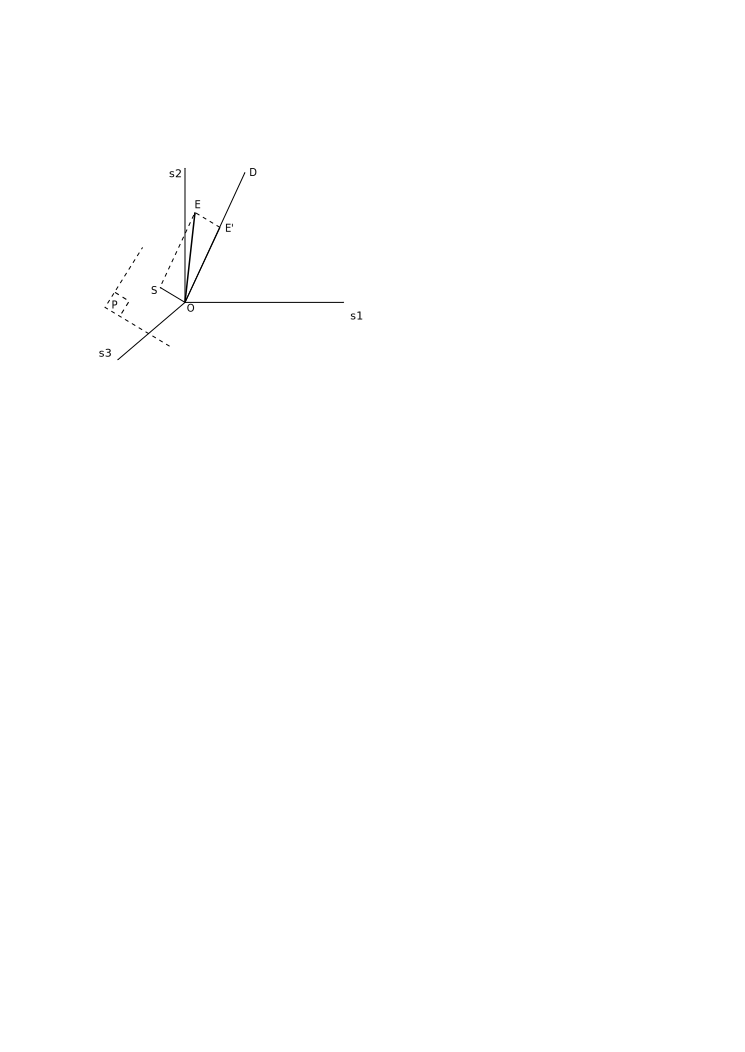
\includegraphics{../images/T1_Ch02-0012}
    \end{center}
\end{wrapfigure}
Cette représentation, très utile, exige néanmoins certaines précautions: on représente géométriquement l'espace des contraintes principales par un espace vectoriel mais ce n'est pas un espace vectoriel.
En particulier, les changements d'axes sont dépourvus de sens.
En particulier également, la somme de deux tenseurs $\sigma_{ij}^{(1)} + \sigma_{ij}^{(2)}$ ne correspond pas à la somme vectorielle (sauf dans le cas où les tenseurs $\sigma_{ij}^{(1)}$ et $\sigma_{ij}^{(2)}$ ont mêmes directions principales).
Enfin, un tenseur des contraintes est représenté, en toute rigueur, non pas par un point, mais par 6 points, car la numérotation des valeurs propres $\sigma_1$, $\sigma_2$, $\sigma_3$ est arbitraire. 

Dans cet espace, les tenseurs sphériques sont représentés par les points de l'«~axe hydrostatique $\Delta$~» (cosinus directeurs: $1/\sqrt{3},\ 1/\sqrt{3},\ 1/\sqrt{3}$).
Les déviateurs sont représentés par les points du plan déviatoire $\Pi$ , perpendiculaire en O à l'axe hydrostatique $\Delta$
\begin{equation}
    \sigma_1 + \sigma_2 + \sigma_3 = 0
    \label{eq:Ch02-027}
\end{equation}
La décomposition~\eqref{eq:Ch02-012} d'un tenseur en partie sphérique et déviateur correspond à la projection orthogonale sur $\Delta$ et $\Pi$.
En particulier, la projection sur $\Delta$ est caractérisée par la trace de $\mathbb{\sigma}$.
Dans le plan déviatoire $\Pi$ on trace 
\begin{center}
    \psfrag{Plan P}{Plan $\Pi$}
    \psfrag{S}{$S$}
    \psfrag{s1}{$\sigma_1$}
    \psfrag{s2}{$\sigma_2$}
    \psfrag{s3}{$\sigma_3$}
    \psfrag{r}{$r$}
    \psfrag{t}{$\theta$}
    \psfrag{h1}{$\vec{h}_1$}
    \psfrag{h2}{$\vec{h}_2$}
    \psfrag{h3}{$\vec{h}_3$}
    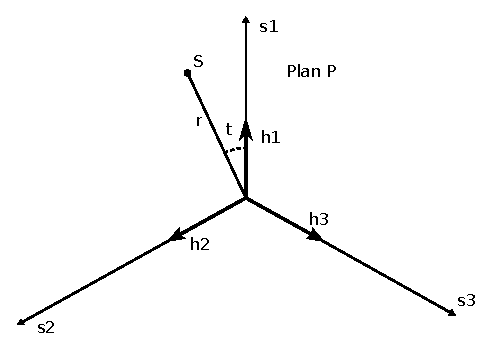
\includegraphics{../images/T1_Ch02-0013}
\end{center}
la projection des axes $O\sigma_1$, $O\sigma_2$, $O\sigma_3$, qui font entre eux un angle de $2\pi/3$ et un tenseur $\mathbb{\sigma}$ sera représenté par le point $S$
\begin{equation}
    \vec{OS} = \sigma_1 \vec{h}_1 + \sigma_2 \vec{h}_2 + \sigma_3 \vec{h}_3
    \label{eq:Ch02-028}
\end{equation}
$\vec{h}_1$, $\vec{h}_2$, $\vec{h}_3$ étant les trois vecteurs unitaires portés par les axes $O\sigma_1$, $O\sigma_2$, $O\sigma_3$ -- ou plutôt par leurs projections, mais nous les notons encore $O\sigma_1$, $O\sigma_2$, $O\sigma_2$, $O\sigma_3$.
En particulier, on vérifie bien que le point $S$ ainsi construit caractérise le déviateur, puisque, si l'on rajoute à $\mathbb{\sigma}$ un tenseur sphérique arbitraire, le point $S$ ne change pas, car $\vec{h}_1 + \vec{h}_2 + \vec{h}_3 = 0$.

On peut alors montrer que la position du point $S$ est complètement caractérisée par les deux invariants $J_2$ et $J_3$ introduits par~\eqref{eq:Ch02-016}.
Plus précisément, un calcul direct montre que les coordonnées polaires $\left( r,\ \theta \right)$ de $S$ sont données par 
\begin{equation}
    r = \sqrt{-3J_2},\ \cos 3 \theta = \frac{3\sqrt{3}}{2}\frac{J_3}{J_2^{3/2}}
    \label{eq:Ch02-029}
\end{equation}
Le second invariant $J_2$ détermine la distance $OS$, c'est à dire «~l'intensité~» du déviateur, tandis que le troisième invariant $J_3$ détermine son orientation. 
Plus précisément, on constate que l'on a 
\begin{align}
    3\theta = \pm \arccos \left( \frac{3\sqrt{3}}{2} \frac{J_3}{J_2^{3/2}} \right) + 2 k \pi\nonumber\\
    \theta &= \pm \frac{1}{3}\arccos \left( \frac{3\sqrt{3}}{2} \frac{J_3}{J_2^{3/2}} \right) + \frac{2 k \pi}{3}
    \label{eq:Ch02-030}
\end{align}
\begin{wrapfigure}[9]{r}{.4\textwidth}
    \begin{center}
        \psfrag{s1}{$\sigma_1$}
        \psfrag{s2}{$\sigma_2$}
        \psfrag{s3}{$\sigma_3$}
        \psfrag{S1}{$S_1$}
        \psfrag{S2}{$S_2$}
        \psfrag{S3}{$S_3$}
        \psfrag{S4}{$S_4$}
        \psfrag{S5}{$S_5$}
        \psfrag{S6}{$S_6$}
        \psfrag{O}{$O$}
        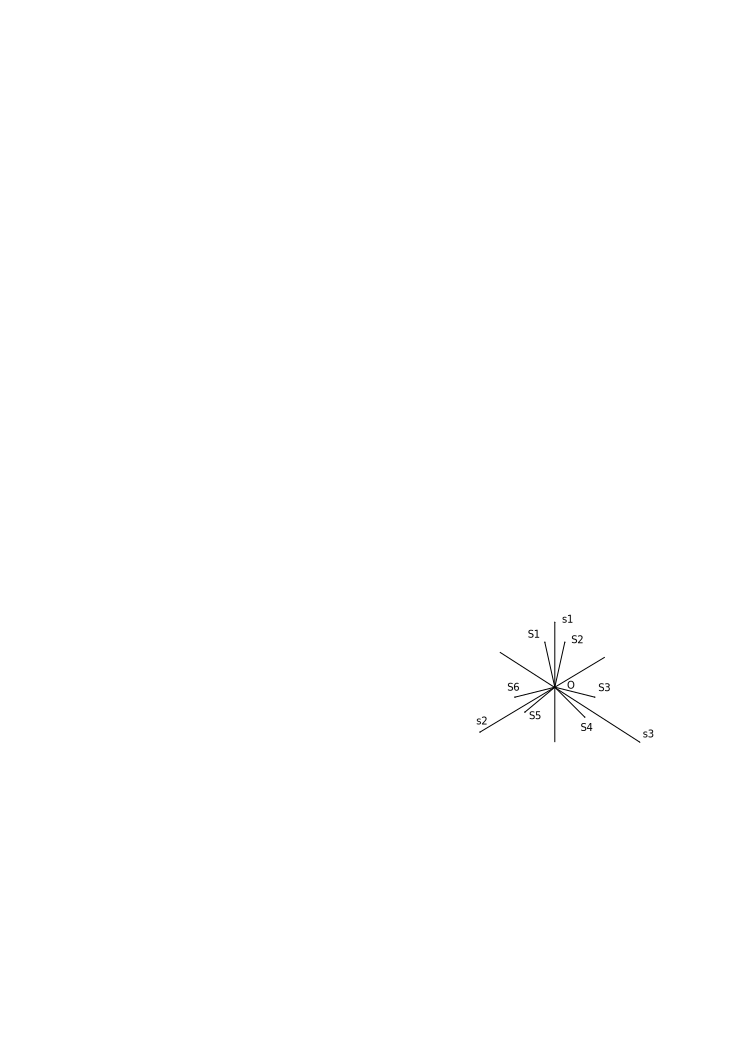
\includegraphics{../images/T1_Ch02-0014}
    \end{center}
\end{wrapfigure}
ce qui donne les 6 points $S$ correspondant aux 6 numérotations possibles des trois valeurs propres. 
Si l'on impose par exemple $\sigma_1 > \sigma_2 > \sigma_3$ alors on se restreint au quartier $O\sigma_1\sigma_3^{\prime}$ et le point $S$ est complètement défini. 

Finalement, on constate que la position du point $\Sigma$ dans l'espace des contraintes principales est complètement caractérisée par $I_1$, $J_2$, $J_3$: $I_1$ fixe la projection sur $\Delta$, $J_2$ la distance à $\Delta$ et $J_3$ l'orientation de la projection de $O\Sigma$ sur $\Pi$.

\section{Représentation de Mohr} \label{sec:Ch02-3}
\subsection{Tricercle de Mohr} \label{ssec:Ch02-3.1}
La représentation de Mohr est une représentation dans le plan des contraintes normales et tangentielles. 
On porte en abscisse la contrainte normale (algébrique) et en ordonnée le module de la contrainte tangentielle.
\begin{center}
    \psfrag{s1}{$\sigma_1$}
    \psfrag{s2}{$\sigma_2$}
    \psfrag{s3}{$\sigma_3$}
    \psfrag{M1}{$M_1$}
    \psfrag{M2}{$M_2$}
    \psfrag{M3}{$M_3$}
    \psfrag{M}{$M$}
    \psfrag{O}{$O$}
    \psfrag{Tt}{$|\vec{T}_t|$}
    \psfrag{Tn}{$T_n$}
    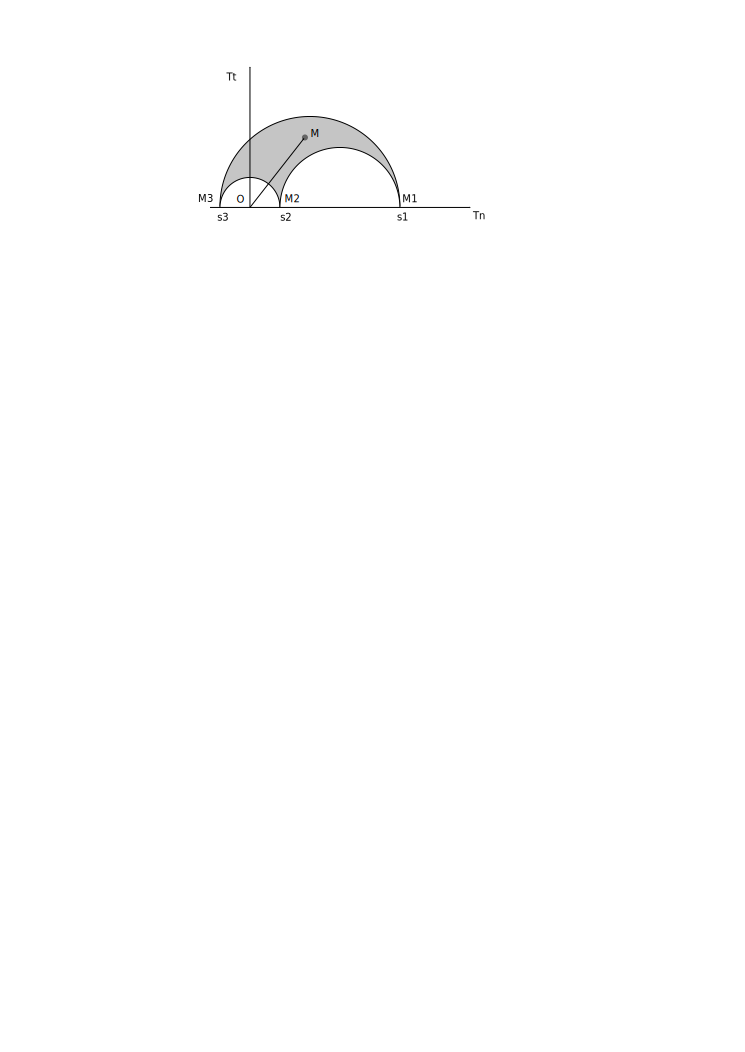
\includegraphics{../images/T1_Ch02-0015}
\end{center}
On obtient ainsi un point $M$ pour chaque facette, et on cherche le lieu de ces points lorsque l'on fait varier la facette.
Pour faire les calculs, on se place en repère principal du tenseur des contraintes et on suppose les valeurs propres rangées par ordre décroissant, $\sigma_3 < \sigma_2 < \sigma_1$.
Les points $M_1$, $M_2$ et $M_3$ correspondant aux facettes normales aux directions principales sont sur l'axe des contraintes normales.
Pour une facette quelconque, on a
\begin{displaymath}
    T_1 = \sigma_1 n_1 \quad T_2 = \sigma_2 n_2 \quad T_3 = \sigma_3 n_3
\end{displaymath}
qui permet de calculer $T_n = T_i n_i$ et $|T|^2 = T_n^2 + T_t^2$
\begin{equation}
    T_n = \sigma_1 n_1^2 + \sigma_2 n_2^2 + \sigma_3 n_3^2
    \label{eq:Ch02-031}
\end{equation}
\begin{equation}
    T_n^2 + T_t^2 = \sigma_1^2 n_1^2 + \sigma_2^2 n_2^2 + \sigma_3^2 n_3^2
    \label{eq:Ch02-032}
\end{equation}
Etant donnée une valeur de $T_n$ et de $T_t$, peut-on trouver une facette qui leur corresponde ?
Pour cela, il faut calculer $n_1$, $n_2$, $n_3$ à partir du système formé par \eqref{eq:Ch02-031}, \eqref{eq:Ch02-032} et la relation 
\begin{equation}
    1 = n_1^2 + n_2^2 + n_3^2
    \label{eq:Ch02-033}
\end{equation}
exprimant le fait que le vecteur $\vec{n}$ est unitaire.
On a donc un système linéaire en $n_1^2$, $n_2^2$, $n_3^2$, dont la solution est 
\begin{equation}
    n_1^2 = \frac{T_t^2 + \left( T_n - \sigma_2 \right)\left( T_n - \sigma_3 \right)}{\left( \sigma_1 - \sigma_2 \right)\left( \sigma_1 - \sigma_3 \right)}
    \label{eq:Ch02-034}
\end{equation}
et $n_2^2$, $n_3^2$, par permutation circulaire.
Géométriquement, on retrouve au dénominateur le produit scalaire $\vec{M_1M_2}\cdot\vec{M_1M_3}$ et au numérateur le produit scalaire $\vec{MM_2}\cdot \vec{MM_3}$.
On a donc 
\begin{equation}
    n_1^2 = \frac{\vec{MM_2} \cdot \vec{MM_3}}{\vec{M_1M_2} \cdot \vec{M_1M_3}},\quad n_2^2 = \frac{\vec{MM_1} \cdot \vec{MM_3}}{\vec{M_2M_1} \cdot \vec{M_2M_3}},\quad n_3^2 = \frac{\vec{MM_1} \cdot \vec{MM_2}}{\vec{M_3M_1} \cdot \vec{M_3M_2}}
    \label{eq:Ch02-035}
\end{equation}
Pour que cette solution soit satisfaisante, il faut vérifier que $n_1^2$, $n_2^2$ et $n_3^2$ sont positifs 
\begin{equation}
    n_1^2 \geq 0, n_2^2 \geq 0, n_3^2 \geq 0, 
    \label{eq:Ch02-036}
\end{equation}
Or, puisque $\sigma_3 < \sigma_2 < \sigma_1$, il est clair que
\begin{equation}
    \vec{M_1M_2} \cdot \vec{M_1M_3} \geq 0, \quad \vec{M_2M_1} \cdot \vec{M_2M_3} \leq 0, \quad \vec{M_3M_1} \cdot \vec{M_3M_2} \geq 0
    \label{eq:Ch02-037}
\end{equation}
Les conditions~\eqref{eq:Ch02-036} exigent donc 
\begin{equation}
    \vec{MM_2} \cdot \vec{MM_3} \geq 0, \quad \vec{MM_1} \cdot \vec{MM_3} \leq 0, \quad \vec{MM_1} \cdot \vec{MM_2} \geq 0
    \label{eq:Ch02-038}
\end{equation}
c'est-à-dire que les angles $\bigl( \vec{MM_2},\vec{MM_3} \bigr)$ et  $\bigl( \vec{MM_1},\vec{MM_2} \bigr)$ soient aigus et que l'angle $\bigl( \vec{MM_1}, \vec{MM_3} \bigr)$ soit obtus, c'est-à-dire, encore, que le point $M$ soit à l'extérieur des deux demi-cercles de diamètres $M_1M_2$ et $M_2M_3$, et à l'intérieur du demi-cercle de diamètre $M_1M_3$.
Ainsi, quand $\vec{n}$ varie, le point $M$ reste dans la surface hachurée appelée -- tricercle de Mohr -- et qui devient un demi cercle si deux valeurs propres coïncident, et un point pour un tenseur sphérique.

On constate d'autre part que $M$ décrit le demi cercle de diamètre $M_1M_3$ lorsque $\vec{n}$ varie dans le plan $\vec{e}_1, \vec{e}_3$ (car \eqref{eq:Ch02-035} montre que $n_2 = 0$  si et seulement si $\vec{MM_1}$ est orthogonal à $\vec{MM_3}$).
On voit également que le maximum de la contrainte de cisaillement (lorsque l'on fait varier la facette) est égale au rayon du plus grand cercle, c'est à dire à la demi différence des contraintes principales extrêmes
\begin{equation}
    |T_t|_{max} = \frac{\sigma_1 - \sigma_3}{2} = \frac{1}{2} \max_{i,j} |\sigma_i - \sigma_j|
    \label{eq:Ch02-039}
\end{equation}
On montrera au paragraphe~\ref{ssec:Ch02-3.2} que ce maximum est atteint lorsque $\vec{n}$ est bissectrice des directions principales.  

\subsection{Cercle de Mohr -- Pole} \label{ssec:Ch02-3.2}
Nous considérons maintenant un état plan de contraintes~\eqref{eq:Ch02-022}, et nous faisons varier $\vec{n}$, dans le plan $\bigl( x_1,x_2 \bigr)$.
On peut alors orienter la direction tangentielle à la facette en introduisant un vecteur unitaire $\vec{t}$ à $+\pi/2$ de $\vec{n}$.
La contrainte tangentielle $T_t$ devient donc une quantité algébrique, et la représentation dans le plan de Mohr permet de déterminer l'orientation du vecteur contrainte. 
\begin{multicols}{2}
    \begin{center}
        \psfrag{x1}{$x_1$}
        \psfrag{x2}{$x_2$}
        \psfrag{x1'}{$x_1'$}
        \psfrag{x2'}{$x_2'$}
        \psfrag{t}{$\theta$}
        \psfrag{Tt}{$T_t$}
        \psfrag{Tn}{$T_n$}
        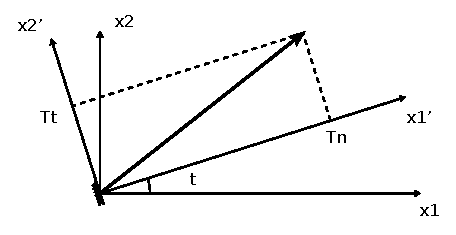
\includegraphics{../images/T1_Ch02-0016a}
    \end{center}
    \columnbreak
    \begin{center}
        \psfrag{Tn}{$T_n$}
        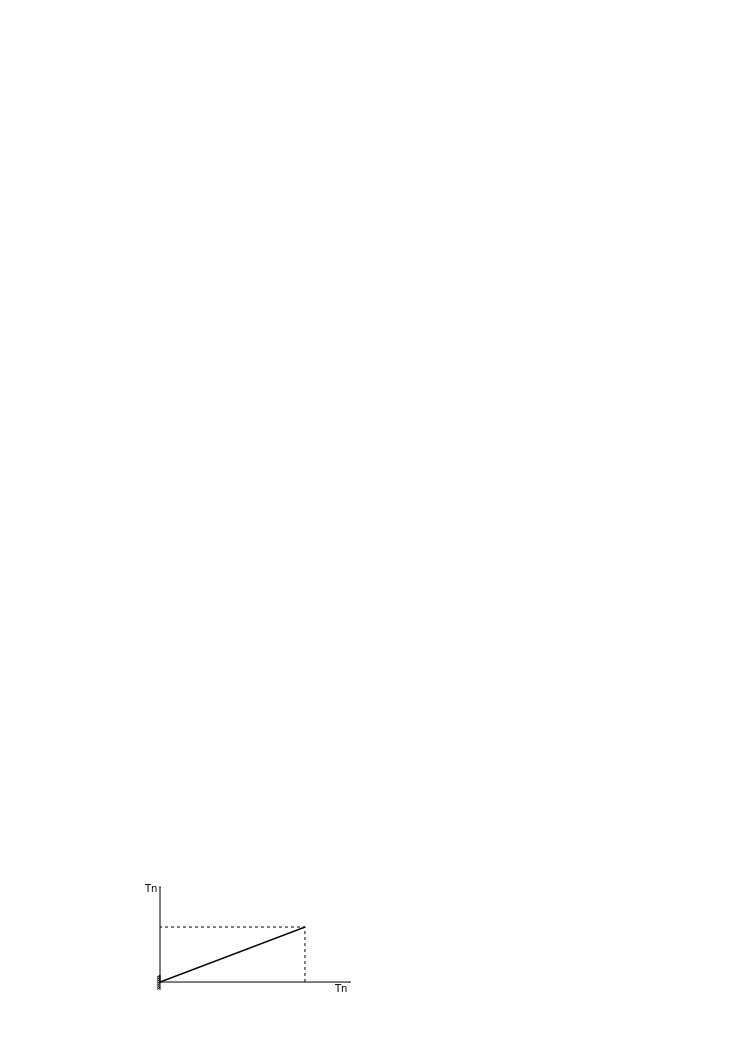
\includegraphics{../images/T1_Ch02-0016b}
    \end{center}
\end{multicols}
Pour calculer $T_n$ et $T_t$ on écrit
\begin{displaymath}
    \vec{n} = 
    \begin{bmatrix}
        \cos \theta\\
        \sin \theta
    \end{bmatrix}
    \quad
    \vec{t} = 
    \begin{bmatrix}
        -\sin \theta
        \cos \theta
    \end{bmatrix}
\end{displaymath}
on calcule le vecteur contrainte
\begin{equation}
    \left\{
    \begin{array}{lll}
        T_1 & = \sigma_{11} \cos \theta & + \sigma_{12} \sin \theta\\
        T_2 & = \sigma_{12} \cos \theta & + \sigma_{22} \sin \theta
    \end{array}
    \right.
    \label{eq:Ch02-040}
\end{equation}
et ensuite et en projetant $T_n$ et $T_t$ sur $\vec{n}$ et $\vec{t}$
\begin{equation}
    \left\{
    \begin{aligned}
        T_n &= \sigma_{11} \cos^2 \theta + 2 \sigma_{12} \cos \theta \sin \theta + \sigma_{22} \sin^2 \theta\\
            &= \frac{\sigma_{11} + \sigma_{22}}{2} + \frac{\sigma_{11} - \sigma_{22}}{2} \cos 2 \theta + \sigma_{12} \sin 2 \theta\\
        T_t &= \left(\sigma_{22}-\sigma_{11}\right) \cos \theta \sin \theta + \sigma_{12} \left( \cos^2\theta -\sin^2 \theta \right)\\
            &= -\frac{\left(\sigma_{11}-\sigma_{22}\right)}{2} + \sigma_{12} \cos 2 \theta
    \end{aligned}
    \right.
    \label{eq:Ch02-041}
\end{equation}
Les directions principales s'obtiennent en annulant la contrainte tangentielle $T_t = 0$:
\begin{equation}
    \tan 2 \theta_0 = \frac{2\sigma_{12}}{\sigma_{11} - \sigma_{22}}
    \label{eq:Ch02-042}
\end{equation}
ce qui définit $\theta_0$ à $k\pi/2$ près.
Nous choisissons $\theta_0$ en posant 
\begin{equation}
    \left\{
    \begin{aligned}
        \sigma_{12} &= \sqrt{\left( \frac{\sigma_{11} - \sigma_{12}}{2} \right)^2 + \sigma_{12}^2} \sin 2 \theta_0 \\
        \frac{\sigma_{11} - \sigma_{22}}{2} &= \sqrt{\left( \frac{\sigma_{11} - \sigma_{12}}{2} \right)^2 + \sigma_{12^2}} \cos 2 \theta_0
    \end{aligned}
    \right.
    \label{eq:Ch02-043}
\end{equation}
En reportant dans \eqref{eq:Ch02-043}, on obtient alors 
\begin{equation}
    \begin{aligned}
        T_n &= \frac{\sigma_{11} + \sigma_{22}}{2} + \sqrt{\left( \frac{\sigma_{11} - \sigma_{22}}{2} \right)^2 + \sigma_{12}^2} \cos 2 \left( \theta_0 - \theta \right)\\
        T_t &= \sqrt{\left( \frac{\sigma_{11} - \sigma_{22}}{2} \right)^2 + \sigma_{12}^2} \sin 2 \left( \theta_0 - \theta \right)
    \end{aligned}
    \label{eq:Ch02-044}
\end{equation}
Lorsque $\theta$ varie, le point $M$, représentant le vecteur contrainte dans le plan $T_n$, $T_t$, décrit un cercle de centre $\Omega$ et rayon $R$
\begin{equation}
    \Omega = \left( \frac{\sigma_{11}+\sigma_{22}}{2}, 0 \right), \ R = \sqrt{\left( \frac{\sigma_{11} - \sigma_{22}}{2} \right)^2 + \sigma_{12}^2}
    \label{eq:Ch02-045}
\end{equation}
\begin{center}
    \psfrag{Tt}{$T_t$}
    \psfrag{Tn}{$T_n$}
    \psfrag{A1}{$A_1$}
    \psfrag{A2}{$A_2$}
    \psfrag{B1}{$B_1$}
    \psfrag{B2}{$B_2$}
    \psfrag{M1}{$M_1$}
    \psfrag{M2}{$M_2$}
    \psfrag{2t}{$2\theta$}
    \psfrag{2t0}{$2\theta_0$}
    \psfrag{s11}{$\sigma_{11}$}
    \psfrag{s12}{$\sigma_{12}$}
    \psfrag{-s12}{$-\sigma_{12}$}
    \psfrag{s22}{$\sigma_{22}$}
    \psfrag{x1}{$x_1$}
    \psfrag{x2}{$x_2$}
    \psfrag{O}{$O$}
    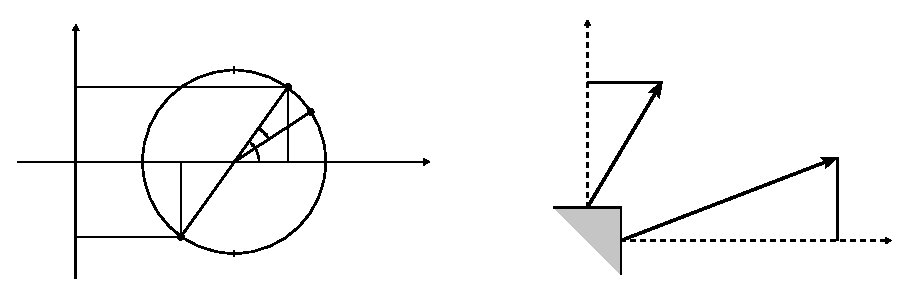
\includegraphics{../images/T1_Ch02-0017}
\end{center}
Les points  et $M_1\ \left( \sigma_{11},\ \sigma_{12} \right)$ et $M_2\ \left( \sigma_{22},\ -\sigma_{12} \right)$ correspondent à $\vec{n} = \vec{e}_1$ et $\vec{n}=\vec{e}_2$ respectivement. 
Pour obtenir le point $M$ correspondant à une normale $\vec{n}$ formant un angle $\theta$ avec $\vec{e}_1$, il faut tourner par rapport à $\Omega M_1$ d' un angle $2\theta$ dans le sens rétrograde.
Les points $A_1$ et $A_2$ correspondent aux directions principales, $\theta = \theta_0 + k\pi/2$ et les contraintes principales sont données par 
\begin{equation}
    \sigma_{1\text{ ou }2} = \frac{\sigma_{11} + \sigma_{22}}{2} \pm \sqrt{\left( \frac{\sigma_{11} - \sigma_{22}}{2} \right)^2 +\sigma_{12}^2}
    \label{eq:Ch02-046}
\end{equation}
Les points $B_1$ et $B_2$ correspondent aux directions de cisaillement maximal et sont donnés par $\theta = \theta_0 + \pi/4 + k\pi/2$, ce sont donc les bissectrices des directions principales, comme annoncé à la fin du paragraphe~\ref{ssec:Ch02-3.1}. 

Le point $M_1$ est appelé pôle du cercle de Mohr, et il permet une construction graphique du vecteur contrainte associé à une facette quelconque.
\begin{center}
    \psfrag{Tt}{$T_t$}
    \psfrag{Tn}{$T_n$}
    \psfrag{A1}{$A_1$}
    \psfrag{A2}{$A_2$}
    \psfrag{B1}{$B_1$}
    \psfrag{B2}{$B_2$}
    \psfrag{M}{$M$}
    \psfrag{M'}{$M'$}
    \psfrag{M1}{$M_1$}
    \psfrag{M1'}{$M_1'$}
    \psfrag{M2}{$M_2$}
    \psfrag{t}{$\theta$}
    \psfrag{2t}{$2\theta$}
    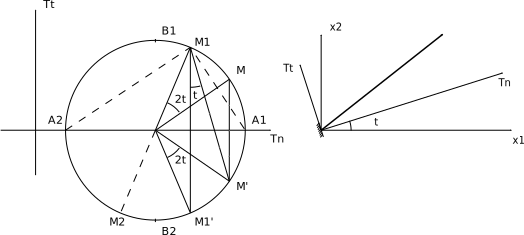
\includegraphics{../images/T1_Ch02-0018}
\end{center}
Pour obtenir le point $M$, c'est à dire le vecteur contrainte s'exerçant sur une facette inclinée de $\theta$ par rapport à la verticale, on utilise la construction suivante.
\begin{enumerate}
    \item On trace $M_1 M^{\prime}$ parallèle à la facette considérée, qui coupe le cercle de Mohr en $M^{\prime}$.
    \item $M$ est le symétrique de $M^{\prime}$ par rapport à l'axe des $T_n$.
\end{enumerate}
On en tire en particulier les directions principales $M_1 A_1$ et $M_1 A_2$ ainsi que les directions de contrainte tangentielle maximum $M_1 B_1$ et $M_1 B_2$. 

